\documentclass[../main.tex]{subfiles}

\begin{document}
In diesem Kapitel werden die physikalische Vorgänge des Versuches beschrieben. 
Die gegebenen Massen sind:
\begin{itemize}
	\item Gewicht[m] = 2kg
	\item Velocity[v] = 2m/s
	\item Würfelseite = 1.5m
\end{itemize}
\subsection{Lab 2: Würfel bewegt sich und stösst}
Es werden drei Vorgänge beschrieben, die Beschleunigung durch die konstante Kraft, einen elastischen Stoss und einen inelastischen Stoss.
Ein Würfel, namens Romeo, wird durch die konstante Kraft beschleunigt, bis maximal eine Geschwindigkeit von 2m/s erreicht wird.
Romeo trifft auf eine Feder zu, die an eine Wand befestigt ist.
Dabei geschieht ein elastischer Stoss und der Würfel gleitet wieder zurück und stösst dabei einen zweiten Würfel,
Julia, diesmal passiert der Stoss inelastisch. Sämtliche Vorgänge erfolgen ohne Reibungskräfte.
\subsubsection{Konstante Kraft}
Um die konstante Kraft zu berechnen nehmen wir die gewünschte Geschwindigkeit und berechnen damit die Beschleunigung,
weil die Kraft sowohl von der Masse wie auch der Beschleunigung abhängt und
gegeben ist durch die Formel\cite{tiplerpaula.PhysikFurStudierende}
\begin{mdframed}
		 $F = m*a$
\end{mdframed}
Um dieses Anfangwertproblems zu lösen leiten wir die Geschwindigkeit ab\cite{tiplerpaula.PhysikFurStudierende}:
\begin{mdframed}
		 $\dot{v} = a$\\
$2m*s^{-1} \rightarrow$  $-2m*s^{-2} \rightarrow$  $a = [\frac{2m}{s^{2}}]$
\end{mdframed}
Die Zeit, die gebraucht wird um den Würfel zu beschleunigen, wird durch folgende Formel
beschrieben \cite{tiplerpaula.PhysikFurStudierende}:
\begin{mdframed}
 $v=a*t \rightarrow$ $t=\frac{v}{a} \rightarrow$ $\frac{2m/s}{2m/s^{2}} = 1s$
\end{mdframed}
Somit können wir nun die Kraft ausrechnen:
\begin{mdframed}
$F = 2kg * \frac{2m}{s^{2}} => \frac{4kg*m}{s^{2}} = 4N$
\end{mdframed}
4N werden deshalb als konstante Kraft angewendet, damit auch die gewünschte Geschwindigkeit
erreicht wird, danach wird keine Kraft mehr hinzugefügt und Romeo gleitet auf die Feder zu.
\newpage
\subsubsection{Elastischer Stoss}
Beim elastischen Stoss ist die kinetische Energie vom Stosspartner vor und nach der Kollision
gleich \cite{tiplerpaula.PhysikFurStudierende}. Gemäss Auftrag wird die Federlänge und Federkonstante
so dimensioniert, dass der Würfel nicht auf die Wand trifft.
Die kinetische Energie des Würfels wird mit folgender Formel berechnet \cite{tiplerpaula.PhysikFurStudierende}:
\begin{mdframed}
$E_{kin_{Romeo}}=\frac{1}{2} * m * v^{2}$
\end{mdframed}
Setzt man die Massen von diesem Projekt ein erhält man:
\begin{mdframed}
$\frac{1}{2} * 2kg * (\frac{2m}{s})^{2} = 4J$
\end{mdframed}
Während des Stosses wird die kinetische Energie auf die Feder übetragen. Die Feder speichert diese
Energie in Form von potentieller Energie, da sie zusammenngedrückt wird. Sobald sie Romeo zurück
stösst, wird diese Energie in eine kinetische zurückgewandelt.\newline
Um die Federkonstante zu berechnen, nehmen wir die Tatsache der Energieerhaltung zu Nutze und
setzen die ausgerechnete kinetische Energie gleich mit der potentiellen Energie der Feder.\newline
Die Formel für die pontentielle Energie der Feder lautet\cite{tiplerpaula.PhysikFurStudierende}:
\begin{mdframed}
$E_{pot_{Feder}}=\frac{1}{2} * k * x^{2}$
\end{mdframed}
Die Gleichsetzung der Energien, sieht folgendermassen aus\cite{tiplerpaula.PhysikFurStudierende}:
\begin{mdframed}
$E_{kin_{Romeo}}=E_{pot_{Feder}}$\\\\
$\frac{1}{2} * m * v^{2} = \frac{1}{2} * k * x^{2}$
\end{mdframed}
Diese Gleichung stellen wir um und lösen nach der Federkonstante k auf:
\begin{mdframed}
$ k=\frac{m * v^{2}}{x^{2}}$
\end{mdframed}
Mit den eingesetzen Massen und die gewählte maximale Auslenkung erhalten wir:
\begin{mdframed}
$\frac{2kg*(2m/s)^{2}}{(1.7m)^{2}} = 2.77N/m$
\end{mdframed}
Jetzt wo wir die Federkonstante und Länge haben, können wir einen langsamen Stoss gewährleisten.
\newpage
\subsubsection{Inelastischer Stoss}
Beim vollständigen inelastischen Stoss, werden beide Stosspartner nach der Kollision verbunden sein und dieselbe
Geschwindigkeit haben \cite{tiplerpaula.PhysikFurStudierende}. Die Formeln, die wir für diesen Vorgang brauchen sind,
die der Impulse der beiden Körper:
\begin{mdframed}
$Impuls_{Romeo} = m_{Romeo}*v_{Romeo} = 2kg * 2m/s = 4 Ns$\\\\
$Impuls_{Julia} = m_{Julia}*v_{Julia} = 2kg * 0m/s = 0Ns$
\end{mdframed}
 Bei diesem Vorgang wird ein Teil des Impulses von Romeo auf Julia übertragen. Der Gesamtimpuls bleibt vor
 und nach dem Stoss erhalten und wird durch den Impulserhaltungsatz beschrieben:%\cite{tiplerpaula.PhysikFurStudierende}:
\begin{mdframed}
$Gesamtimpuls = Impuls_{Romeo} + Impuls_{Julia}$
\\\\$m_{Romeo}*v_{Romeo} +  m_{Julia}*v_{Julia} = (m_{Romeo} + m_{Julia})*v_{Ende}$\\\\
$Gesamtimpuls = 4Ns + 0Ns = 4Ns$
\end{mdframed}
Die Endgeschwindigkeit ist die Geschwindigkeit, die beide Körper gemeinsam haben nach dem Stoss.
 Bei diesem Vorgang wird ein Teil des Impulses von Romeo auf Julia übertragen. Der Gesamtimpuls bleibt erhalten vor
 und nach dem Stoss und wird durch den Impulserhaltungsatz beschrieben:\cite{tiplerpaula.PhysikFurStudierende}:
\begin{mdframed}
$v_{Ende} = \frac{Gesamtimpuls}{(m_{Romeo} + m_{Julia})}$\\\\
$v_{Ende} = \frac{4Ns}{2kg + 2kg} = 1m/s$
\end{mdframed}

Die Relation zwischen der kinetischen Energie und des Impulses, können wir folgendermassen
herleiten %\cite{tiplerpaula.PhysikFurStudierende}:
\begin{mdframed}
$E_{kin}=\frac{1}{2} * m * v^{2} = \frac{(mv)^{2}}{2m} = \frac{p^{2}}{2m}$
\end{mdframed}
Wenden wir dies nach dem Stoss an, sehen wir, dass die kinetische Energie geringer wird:
\begin{mdframed}
$E_{kin_{Ende}}=\frac{p^{2}}{2(m_{Romeo} + m_{Julia})} $
\end{mdframed}

\subsection{Teil 3: Beide Würfel schwingen gedämpft}
Bei diesem Versuch spielen gleich mehrere Kräfte eine Rolle um eine gedämpfte Schwingung zu verursachen. Zum einen die Gewichtskraft und zum anderen die Reibungskraft der turbulenten viskosen Luftreibung, die zusammen die Zentripetalkraft ergeben.
Neben den bestehenden bekannten Grössen aus Versuch Lab 2 kommen folgende Grössen hinzu:
\begin{itemize}
	\item R = Seillänge 6m
	\item $c_w$ = 1.1
	\item $\rho_{Luft}$ = $1.2kg/m^3$
	\item g = $9.81 m/s^2$
	\item A = Stirnfläche Würfel = 1.5*1.5 = 2.25
In den folgenden Beispielrechnungen werden die Zahlen genommen für den Würfel Romeo, wobei dasselbe gilt für den Würfel Julia. 	Hinzukommnt, dass in C\# die Cosinus, Sinus und Arctangens im Bogenmass berechnet werden, also werden sie in diesem Kapitel auch so aufgeführt.
\end{itemize}
     \begin{figure}[H]
               \begin{center}
                   \centerline{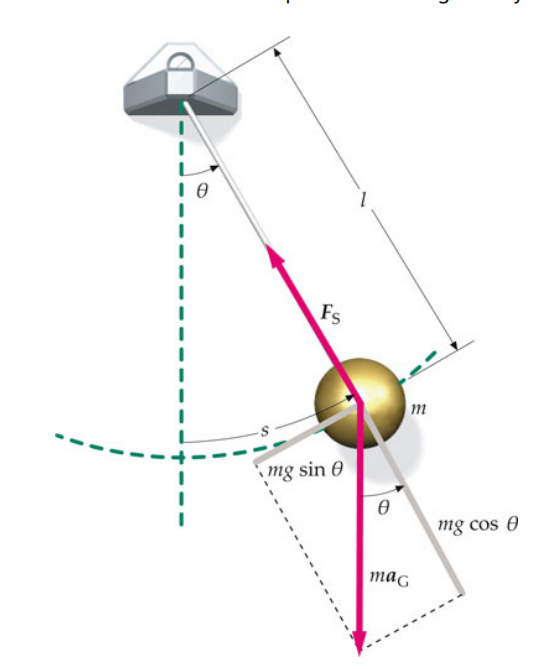
\includegraphics[width=155mm]{./images/Lab3Unity/KraeftePendel.png}}
                   \caption{Kräfte auf eine Pendelmasse \cite{tiplerpaula.PhysikFurStudierende}}
                   \label{fig:Pendel}
               \end{center}
     \end{figure}
\subsubsection{Radialer Anteil der Gewichtskraft}
Die Gewichtskraft ist die Kraft, die durch die Wirkung der Gravitation, auf den Körper wirkt. In einer Schwingung wird der Winkel in der Formelberechnung mitberücksichtigt, da die Punktmasse tangential beschleunigt wird.\cite{tiplerpaula.PhysikFurStudierende}
\begin{mdframed}
$F_g = m * g * cos(\alpha)$
\end{mdframed}
\textbf {Aus dem Versuch:}
\begin{mdframed}
$F_g = 2 * 9.81 * cos(0) = 19.62N$
\end{mdframed}
\subsubsection{Zentripetalkraft}
Diese Kraft ist dem radialen Vektor entgegengesetzt,vorausgesetzt dieser Vektor zeigt vom Kreismittelpunkt nach aussen. Die positive Richtung zeigt demnach nach innen. Diese Kraft ist die Komponente vom resultierenden Kraft, die Senkrecht zur Schwingung steht und zum Mittelpunkt weist. In diesem Fall wird sie durch die Gravatationskraft und die Reibungskraft hervorgerufen und ist somit keine eigenständige neue Kraft.
Die Zetriptalkraft hat die allgemeine Formel \cite{tiplerpaula.PhysikFurStudierende}:
\begin{mdframed}
$F_z=m * \frac{v^2}{R} $
\end{mdframed}
\textbf {Aus dem Versuch:}
\begin{mdframed}
$F_z = 2 * \frac{1.004936^2}{6} = 0.17N$
\end{mdframed}
Wie erwähnt, hängt die Zentripetal Kraft von mehreren Kompenenten ab, in der horizontalen Richtung und in der vertikalen Richtung. Aus diesem Grund werden die horizontalen und vertikalen Komponenten aus den Ortsvektoren zu x und y der Zentripetalkraft zur Gewichtskraft addiert und dann jeweils gemäss der Lehre der Trigonometrie multipliziert mit dem Sinus oder Cosinus des Winkels. Die folgelnde Skizze stellt den Sachverhalt dar:
     \begin{figure}[H]
               \begin{center}
                   \centerline{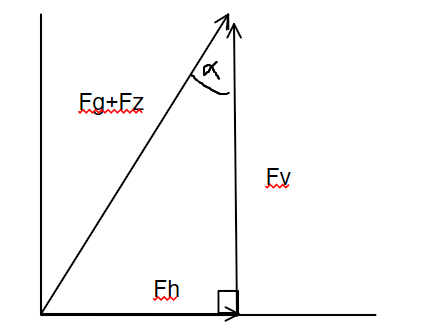
\includegraphics[width=155mm]{./images/Lab3Unity/KraefteDiagramm.png}}
                   \caption{Kräftediagramm Skizze}
                   \label{fig:KräfteDiagramm}
               \end{center}
     \end{figure}
\begin{mdframed}
$H = F_z +F_g$\\\\
$arctan(\alpha)$ = $\frac{Aufhaengepunktseil.x-Position Wuerfel.x }{Aufhaengepunktseil.y-Position Wuerfel.y }$\\\\
$\frac{A}{H}= cos(\alpha) \rightarrow A = (F_z + F_g) * cos(\alpha)= F_v$\\\\
$\frac{G}{H}= sin(\alpha) \rightarrow G = (F_z + F_g) * sin(\alpha)= F_h$\\\\
$Kraftvektor: (Fh,Fv,0)$
\end{mdframed}
\textbf {Aus dem Versuch:\\}
Aufhaengepunktseil so gewaehlt dass Betrag des Vektors 6 ergibt, und bei Winkel 0 also steht der Wuerfel direkt unter dem Aufhaengepunkt, so ergibt es fuer x und z Koordinaten null und zu y beim Aufhaengepunkt 6 dazu addieren.\\
Position Würfel = $(-20.01,5.04,-1.5)$\\
Aufhängepunkt = $(-20.01,11.04,-1.5)$\\
Differenzvektor = $(0,6,0)$\\
\begin{mdframed}
$H = 0.17N +19.62N = 19.77$\\\\
$arctan(0)$ = $\frac{0}{0} = 0$\\\\
$\frac{A}{H}= cos(0) \rightarrow A = (0.17N +19.62N) * cos(0)= 19.77$\\\\
$\frac{G}{H}= sin(0) \rightarrow G = (0.17N +19.62N) * sin(0)= 0$\\\\
$Kraftvektor: (19.77,0,0)$
\end{mdframed}
\subsubsection{Reibungskraft}
Gemäss Aufgabenstellung widerfährt den Würfeln noch eine turbulente viskose Reibungskraft.Die Dampfüng wird durch die Reibungskraft verursacht, denn diese entzieht dem schwingendem System mechanische Energie, die wiederum in Wärmeenergie dissipiert. Diese Kraft errechnet sich aus der Formel:
\begin{mdframed}
$F_r = -0.5 * A*\rho_{Luft}*c_w*v^2*\vec{e_v}$
\end{mdframed}
\textbf {Aus dem Versuch:}
\begin{mdframed}
$F_r = -0.5 * 2.25*1.2kg/m^3*1.1*1.004936^2*(-1.00, 0.00, 0.00) = (1.5,0,0)$
\end{mdframed}
\subsubsection{Resultierende Kraft}
Zu allerletzt wird die vorher berechnete Kraft tangential zur Richtung Geschwindigkeit $\vec{e_v}$ dazu addiert und ergibt die resultierende Kraft, die auf die Würfel gesamthaft wirkt.
\begin{mdframed}
$(Fh,Fv,0) + F_r$
\end{mdframed}
\textbf {Aus dem Versuch:}
\begin{mdframed}
$(19.77,0,0 + (1.5,0,0) = (21.27N,0,0)$
\end{mdframed}
\end{document}